\only<1>{

	\framesubtitle{Attention Space}

	\begin{itemize}

		\item “Dynamics of the \textbf{Law of Small Numbers}, dividing the attention space among factions […] a struggle for attention” \citep[158-160]{collins1994}

		\item "In any period of creative life, there are typically between three and six [...] lineages or schools" \citep[157]{collins1994}

	\end{itemize}

	\vfill

	$\bm{H}$: When the \textbf{density of subfields} within a field surpasses six, the field is more likely to experience a tendency towards \textbf{consolidation}.

}

% \only<2>{

% 	\framesubtitle{Moving Frontier}

% 	\begin{itemize}

% 		\item "High-consensus rapid-discovery science" \citep[157]{collins1994}

% 		\item \textbf{"Fast moving research front"} \citep[158]{collins1994}

% 		\item "\textbf{Ready made} science" v. "Science \textbf{in the making}" \citep{latour1988}

% 	\end{itemize}

% 	\vfill

% 	$\bm{H_{2}}$: \textbf{"Hard" sciences} have a \textbf{faster moving "research front"} than "soft" sciences.

% }

% \only<3>{

% 	\framesubtitle{Research Technology}

% 	\begin{itemize}

% 		\item What sets appart "\textbf{high-consensus rapid-discovery}" from "\textbf{low-consensus non-rapid-discovery}" science? \citep[158]{collins1994}

% 		\item Not "empiricism", "measurement precision", "formalization", or the "experimental method" \citep[158]{collins1994}

% 		\item "\textbf{Genealogy of research technology}" producing reliable observation \citep[158]{collins1994}

% 	\end{itemize}

% 	\vfill

% 	$\bm{H_{3a}}$: A \textbf{change in "research technologies"} should change the structure of the \textbf{"hard" sciences}, while these changes should be absent altogether in "soft" sciences.
% }

% \only<4>{

% 	\framesubtitle{Social conditions \citep{collins1994}}



% 	% E.g.,
% 	% Geopolitics: 9/11
% 	% Economics: 2008 Financial Crisis

% 	“\textbf{Political and economic conditions} change [the] \textbf{material bases} supporting intellectual life, [they] provoke [the] \textbf{realignment of factions”} \citep[165]{collins2000}
	
% 	\vfill

% 	$\bm{H_{3b}}$: A \textbf{change in social or political conditions} should change the structure of the \textbf{"soft" sciences}, while these changes should be absent altogether in "hard" sciences.

% }

\only<2>{

	\framesubtitle{Scientific Revolutions \citep{kuhn2012}}

	\begin{itemize}

		% In Kuhn's model, sciences go through periods of relative stability (i.e., "normal" or "paradigmatic" science) 

		% Anomalies accumulate.

		% Anomalies are observation that do not fit the current models

		% As anomalies accumulate

		% New paradigms emerge and compete

		% Scientific revolution ends when consensus is reached

		% Compares them to political revolutions
		% One institution must die for the next one to be born

		% Basis of science is community consensus (e.g., textbook, curriculums, etc.)

		\item “Political revolutions aim to change political institutions in ways that those institutions themselves prohibit […] necessitates the partial relinquishment of one set of institutions in favor of another […] Initially it is crisis […] that attenuates the role of political institutions […] and the role of paradigms” \citep[93]{kuhn2012}

		\item "Recurrent debates about whether one or another of the contemporary \textbf{social sciences is really a science} [...] will cease to be a source of concern not when a definition is found, but when the groups that now doubt their own status \textbf{achieve consensus} about their past and present accomplishments” \citep[161]{kuhn2012}

	\end{itemize}
	
	\vfill

	$\bm{H}$: Disciplines generally exhibit \textbf{stability}, with occasional episodes of significant \textbf{changes}.

}

\only<3>{

	\framesubtitle{Self-Similarity \citep{abbott2001}}

	\begin{itemize}

		\item “Fractal pattern of division and convergence” \citep{abbott2001}

		\item “The quantitative – qualitative distinction repeats itself at each more detailed level even as the difference between positions narrows” \citep{harty2004}

	\end{itemize}

	\begin{figure}[H]
	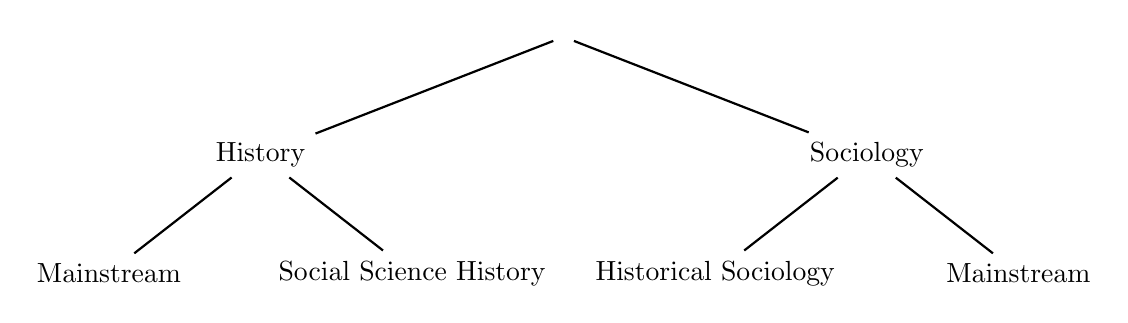
\begin{tikzpicture}[thick,level/.style={sibling distance=77mm/#1}]
	\node [] (r) {}
	  child {
	    node [] (a) {History}
	    child {
	      node [] {Mainstream}
	    }
	    child {
	      node [] {Social Science History}
	    }
	  }
	  child {
	    node [] {Sociology}
	    child {
	      node [] {Historical Sociology}
	    }
	    child {
	      node [] {Mainstream}
	    }
	  };
	\end{tikzpicture}
	\caption{Fractal Distinctions} 
	\label{fig:fractal_distinctions}
\end{figure}

	\vfill

	$\bm{H}$: Within the field, subfields arise, exhibiting a replication of the core structure and retaining distinct features of the broader discipline.

}

\only<4>{

	\framesubtitle{Diffusion \citep{mullins1973}}

	\begin{itemize}

		\item “Successful cluster pays for its success by ceasing to exist [and] scattering” \citep[24]{mullins1973}

		\item “Routinization” and "Institutionalization" \citep{ben-david1960, ben-david1966}

	\end{itemize}

	% \begin{figure}[H]
	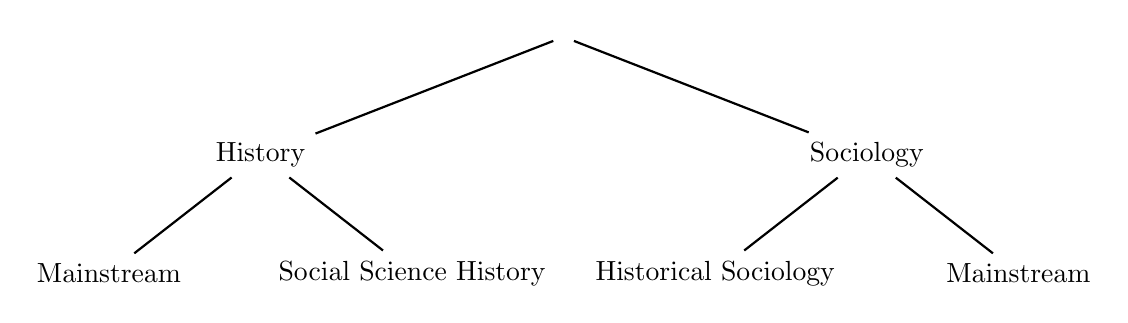
\begin{tikzpicture}[thick,level/.style={sibling distance=77mm/#1}]
	\node [] (r) {}
	  child {
	    node [] (a) {History}
	    child {
	      node [] {Mainstream}
	    }
	    child {
	      node [] {Social Science History}
	    }
	  }
	  child {
	    node [] {Sociology}
	    child {
	      node [] {Historical Sociology}
	    }
	    child {
	      node [] {Mainstream}
	    }
	  };
	\end{tikzpicture}
	\caption{Fractal Distinctions} 
	\label{fig:fractal_distinctions}
\end{figure}

	\vfill
	
	$\bm{H}$: The diffusion of concepts should be apperent in these fields.

}


% % of articles each year that use a term

% % Communities around technologies & ideas 
% % Reliable expected results





% \only<1>{
% 	\framesubtitle{Science as High Consensus, Rapid Discovery Science}
% 	\begin{itemize}

% 		\item "\textbf{Consensus} is not the prevailing pattern [...] \textbf{disagreement} is the norm" \citep[157]{collins1994}

% 		\item What sets appart "\textbf{high-consensus rapid-discovery}" from "\textbf{low-consensus non-rapid-discovery}" science? \citep[158]{collins1994}

% 		\item Not "empiricism", "measurement precision", "formalization", or the "experimental method" \citep[158]{collins1994}

% 		\item "\textbf{Genealogy of research technology}" producing reliable observation \citep[158]{collins1994}

% 		\item Fast moving research front 158

% 		\item "\textbf{Ready made} science" v. "Science \textbf{in the making}" \citep{latour1988}

% 		\item "intensive research goes for the fundamental laws, extensive research goes for the explanation of phenomena in terms of known fundamental laws" \citep[393]{anderson1972}

% 	\end{itemize}
% }

% \only<2>{
% 	\framesubtitle{Science as Attention Space}
% 	\begin{itemize}
% 		\item "In any period of creative life, there are typically \textbf{between three and six [...] lineages or schools}" \citep[157]{collins1994}.
% 		\item "\textbf{Law of Small Numbers}, dividing the \textbf{attention space} among factions" \citep[158]{collins1994}
% 	\end{itemize}
% }

% \only<3>{
% 	\framesubtitle{Science as Revolutionary}
% 	\begin{itemize}
% 		\item "Intellectual \textbf{crisis}, followed by restructuring [...] reduces the number of lineages to the normal ceiling" \citep[157]{collins1994}.
% 		\item During "\textbf{normal science}" "\textbf{anomalies accumulate}"  leading to a phase of "\textbf{revolutionary science}" and a "\textbf{paradigm change}" \citep{kuhn2012}
% 	\end{itemize}
% }

% \only<4>{
% 	\framesubtitle{Science as Technology}
% 	\begin{itemize}
% 		\item "Intellectual community consists in networks that pass \textbf{ideas} [...], research \textbf{technologies} comprise a parallel set of networks" \citep[164]{collins1994}
% 		\item "Human and machine networks develop symbiotically" \citep[164]{collins1994}
% 		\item "\textbf{Human} and \textbf{non-human} network actors" \citep{latour1988}
% 	\end{itemize}
% }

% \only<5>{
% 	\framesubtitle{Science as Institution}
% 	\begin{itemize}
% 		\item "Research equipment, once \textbf{routinized}, may be exported from the laboratory" \citep[165]{collins1994}
% 		\item "Technological \textbf{routine}" \citep[165]{collins1994}
% 		\item “Political \textbf{revolutions} aim to change political institutions in ways that those institutions themselves prohibit […] necessitates the partial \textbf{relinquishment of one set of institutions} in favor of another” \citep[93]{kuhn2012}
% 		\item “Cluster’s social [structural] change is accompanied by intellectual [content] changes” \citep[22]{mullins1973}
% 	\end{itemize}
% }

% \only<6> {
% 	\framesubtitle{Science as Fractal}

% 	\citep{abbott2001}

% 	% \noindent\includegraphics[width=\linewidth]{figures/fractal_distinctions}

% 	\begin{figure}[H]
	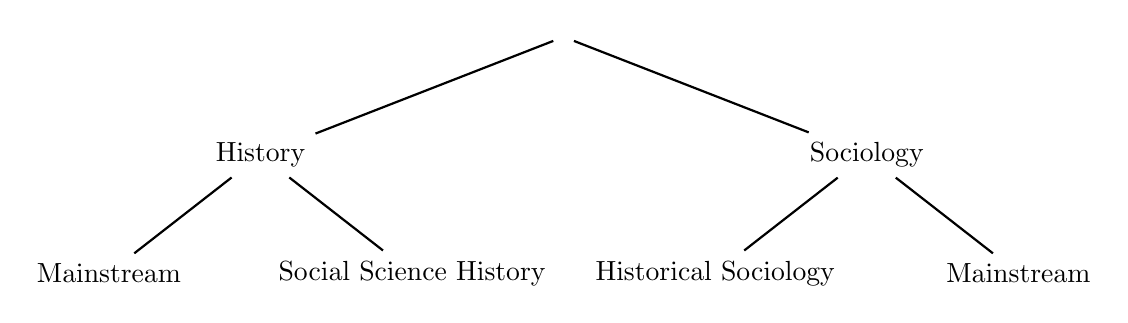
\begin{tikzpicture}[thick,level/.style={sibling distance=77mm/#1}]
	\node [] (r) {}
	  child {
	    node [] (a) {History}
	    child {
	      node [] {Mainstream}
	    }
	    child {
	      node [] {Social Science History}
	    }
	  }
	  child {
	    node [] {Sociology}
	    child {
	      node [] {Historical Sociology}
	    }
	    child {
	      node [] {Mainstream}
	    }
	  };
	\end{tikzpicture}
	\caption{Fractal Distinctions} 
	\label{fig:fractal_distinctions}
\end{figure}

% 	% \begin{figure}
% 	% \begin{tikzpicture}[thick,level/.style={sibling distance=100mm}]
% 	% \node [] (r) {}
% 	%   child {
% 	%     node [] (a) {History}
% 	%     child {
% 	%       node [] {Mainstream}
% 	%     }
% 	%     child {
% 	%       node [] {Social Science History}
% 	%     }
% 	%   }
% 	%   child {
% 	%     node [] {Sociology}
% 	%     child {
% 	%       node [] {Historical Sociology}
% 	%     }
% 	%     child {
% 	%       node [] {Mainstream}
% 	%     }
% 	%   };
% 	% \end{tikzpicture}
% 	% \caption{Fractal Distinctions} 
% 	% \label{fig:fractal_distinctions}
% 	% \end{figure}
% }











